\documentclass{../../handout}
\newcounter{handout}
\renewcommand{\Title}{Mini-dokumentation til Processing.py}%
\renewcommand{\TimeAndLocation}{DIKU, 2018}%
\def\arraystretch{1.5}
\begin{document}
\chapter{Koordinatsystemet}
Koordinatsystemet i Processing har punktet (0,0) i øverste venstre
hjørne, med x-aksen gående mod højre og y-aksen gående nedad. Det er
omvendt hvad vi er vandt til i matematikken hvor y-aksen går opad.
\begin{center}
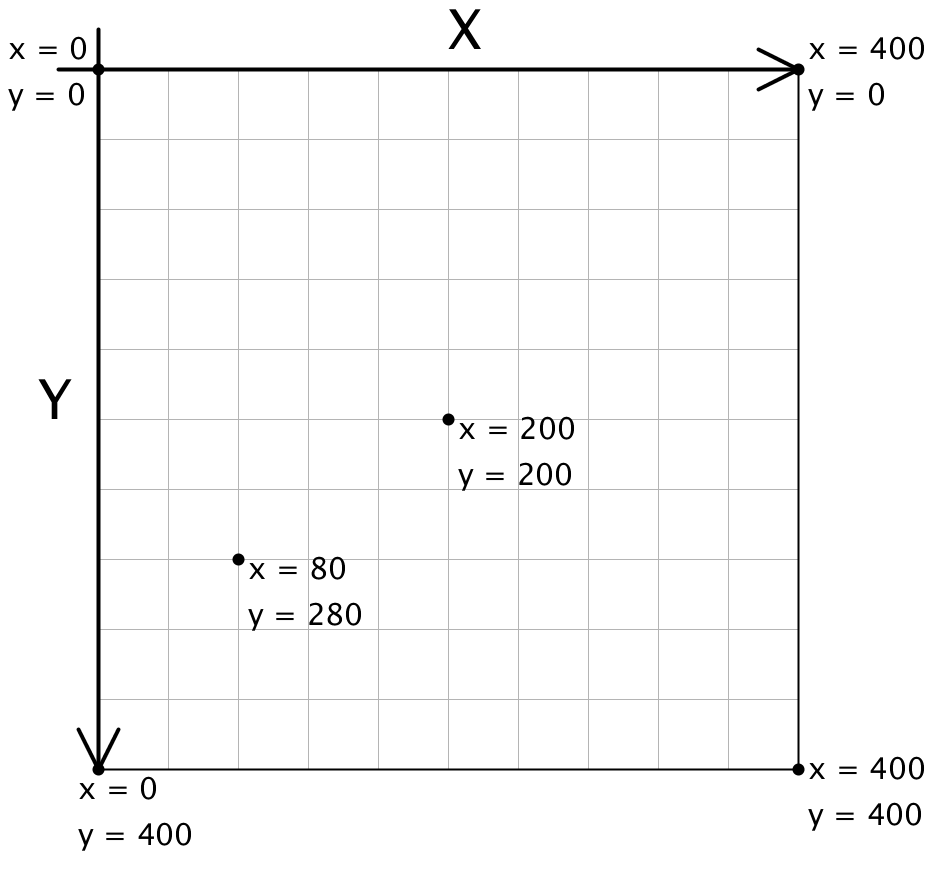
\includegraphics[width=0.7\linewidth, trim={0 7mm 0 0}, clip]{illustrationer/koordinatsystem.png}
\end{center}
\vspace{-6mm}
\chapter{Tegnekommandoer}

\noindent
\begin{tabular}{lp{0.60\linewidth}}
  \ttpy$ellipse(x, y, width, height)$ & Tegn en ellipse. x og y værdier angiver centrum af ellipsen.  \\
  \ttpy$rect(x, y, width, height)$ & Tegn et rektangel. x og y værdierne angiver øverste venstre hjørne. \\
  \ttpy$line(x1, y1, x2, y2)$ & Tegn en linje. \ttpy$x1$ og \ttpy$y1$ angiver den ene ende af linjen. \ttpy$x2$ og \ttpy$y2$ angiver den anden ende af linjen. \\
  \ttpy$triangle(x1, y1, x2, y2, x3, y3)$ & Tegn en trekant. De tre sæt xy-koordinater angiver de tre forskellige hjørner af trekanten. \\
  \ttpy$text("tekst her", x, y)$ & Skriv teksten mellem de to sæt gåseøjne. Teksten tegnes ved det angivne koordinat \\
\end{tabular}

\vspace{1cm}
\hspace{-3cm}
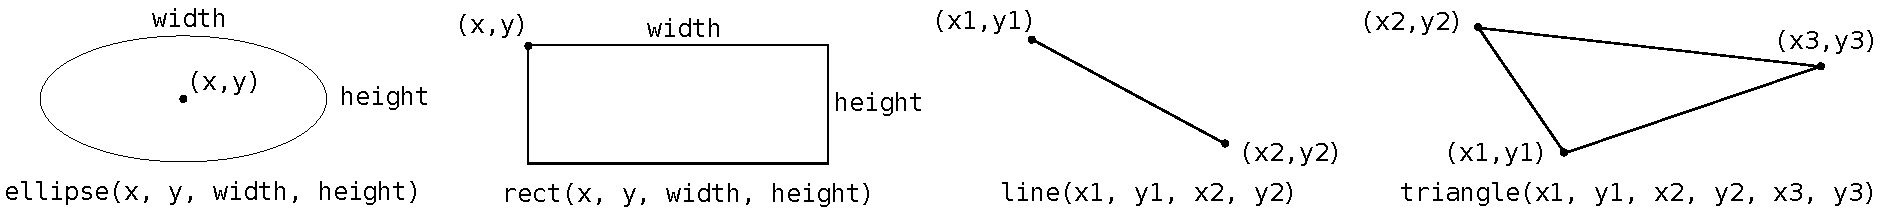
\includegraphics[width=1.5\linewidth]{illustrationer/drawing-commands}


\newpage
\chapter{Farvelægning}
Farver angives som tre værdier i intervallet 0-255 der angiver mængden
af rød, grøn og blå. Det kaldes RGB-farvesystemet. Søg online efter
``rgb color picker'' for at finde værktøjer til at finde farver.

\noindent
\begin{tabular}{lp{0.70\linewidth}}
  \ttpy$background(r, g, b)$ & Slet alt og brug den angivne
                               farve som baggrund  \\
  \ttpy$fill(r, g, b)$ & Angiv udfyldningsfarve. Efterfølgende figurer bliver tegnet i den farve.  \\
  \ttpy$stroke(r, g, b)$ & Angiv omrids-farve. Efterfølgende figurer bliver tegnet med omrids i den farve.  \\
  \ttpy$noStroke()$ & Slå tegning af omrids fra. \\
  \ttpy$noFill()$ & Slå udfyldning af figurer fra, så de er helt gennemsigtige. \\
\end{tabular}

\chapter{Variable}
Definition af variabel:
\begin{python}
x = 4200
\end{python}
Nu kan man bruge \ttpy{x} i sit program i stedet for værdien 4200.

\vspace{2mm}
\noindent
Senere kan variablen ændres:
\begin{python}
x = 17
\end{python}

\noindent
Variablen kan også bruges på højresiden, hvis man fx vil trække 3 fra:
\begin{python}
x = x - 3
\end{python}

\chapter{Funktioner}
\noindent
Definition og kald af funktioner:
\begin{python}
def circleRect(x, y):
    ellipse(x, y, 20, 20)
    rect(x - 10, y - 10, 20, 20)

def scaleAdd(a, b, c):
    temporary = (a * b) + c
    return temporary

# Kald circleRect
# tallene 150 og 100 overføres til funktionen
circleRect(150, 100)

# Kald scaleAdd og aflæs dens returværdi
v = scaleAdd(1000,2,18)
\end{python}
Funktioner kan kalde andre funktioner. Funktioner kan, men behøver
ikke, returnere et resultat via \ttpy{return} keywordet.

\newpage
\chapter{Funktioner med og uden sideeffekter}
Funktionen \ttpy{circleRect} har som \textit{sideeffekt} at tegne en
ellipse og et rektangel på skærmen. Den ændrer på noget udenfor
funktionen. En anden side effekt kunne være at ændre på en variabel
udenfor funktionen (fx en global variabel).

Modsat ændrer \ttpy{scaleAdd} ikke på noget uden for funktionen, den
udfører en beregning og returnerer en værdi. Den har altså ingen
\textit{sideeffekter}.

Det er ikke enten eller, man vil ofte også have funktioner i sit
program der både har sideeffekter og returnerer værdier.


\chapter{Lokale variabler}
En variabel der er defineret inde i en funktion eller som parametre
til en funktion, er lokal for funktionen. Ændrer vi den, påvirker det
ikke noget andre steder i programmet. Se Eksempel 2 nedenfor.

% \begin{python}
% foo = 10
% def eksempel():
%     # Ændrer vi foo her påvirker det ikke "a" deklareret udenfor
%     foo = 20

% eksempel()
% # variablen "foo" er stadig 10 her efter
% \end{python}
% Værdien af variablen \ttpy{foo} er uændret efter eksempel er kørt. Det
% er værdien $10$ der indsættes i funktionen, ikke selve variablen.

\chapter{Globale variabler}
Globale variabler er defineret udenfor funktionerne i programmet. De
behøver ikke gives som argument til funktioner. Hvis man vil ændre på
dem inde i en funktion, er det til gengæld nødvendigt at skrive
\ttpy{global x} i starten af funktionsdefinitionen, for at angive at
den globale variabel \ttpy{x} gerne må ændres.

~

\noindent
Eksempel 1:
\begin{python}
foo = 42
def minfunktion():
    global foo
    foo = 20

minfunktion()
# variablen "foo" er nu sat til 20
\end{python}
Her deklares det at funktionen \ttpy{minfunktion} gerne må ændre i den
globale variabel foo.

~

\noindent
Eksempel 2:
\begin{python}
foo = 42
def minfunktion():
    foo = 20

minfunktion()
# variablen "foo" er stadig 42
\end{python}
Her er der to variabler med samme navn \ttpy{foo}. En global variabel
der har værdien 42, og en lokal variabel der erklæres inde i
funktionen, som tildeles værdien 20. Da der ikke er skrevet
\ttpy{global foo}, vil Python forstå det som om at en ny lokalvariabel
skal oprettes og ``overskygge'' den globale.


\end{document}
